\chapter{Local Correlation: Ground State}

Some choice words here.......

\section{Low-Scaling Hartree Fock Methods}

Talk about bottle necks
DF, CFMM, LinK, CADF, PARI, ...

\subsection{Density Purification}


\section{Local Ground State Correlation Methods: MP2}

Second-Order M{\o}ller Plesset is one of the simplest post-Hartree Fock methods available, but still scales as $\ccpx{5}$. Since the seminal work of Saebo and Pulay (Pul1983,Sae1985), several different methods have been proposed which drastically reduce the computational complexity. Attempts can generally be grouped into two categories: AO-MP2 and LMO-MP2. While both schemes do have their differences, they share some of the problems assciated with computing the MP2 energy in a local basis.

First, the energy denominator in the MP2-amplitudes $t$ make it difficult to reformulate the MP2 energy expressions in a different basis. AO-MP2 and LMO-MP2 take different approaches: AO-MP2 solves the problem using the Laplace quadrature, while LMO-MP2 methods usually use an orbital-invariant formulation of MP2 using the Hylleraas functional.

Second, steps involving the transformation of the AO 2-electron integrals to the Pseudo-AO or LMO basis still remain a major bottle-neck, even with sparsity involved. Both AO- and LMO-MP2 use screening criteria, additional domain restrictions, density fitting or similar methods to lower the cost of integral transformation. These additional procedures are crucial if one wishes to achieve a truly linear scaling MP2 method with a reduced overhead.

We will now address each point in detail in the next sections.

\subsection{Atomic Orbital MP2}

MP2 was first formulated in the AO basis in 1993 by Häser , and a linear scaling algorithm was presented by Scuseria and Ayala in 1999 (ref). AO-MP2 has since then been extended to DF-MP2 (ref) and SOS-MP2 (ref). 

\subsubsection{The Laplace Transform}

In 1991, Almlöf showed (Alm1991) that the energy denominator in the MP2 amplitudes can be removed using an integral transform called the \emph{Laplace Transform}

\begin{equation}
\frac{1}{\eps_a + \eps_b - \eps_i - \eps_j} = \int_0^{\infty} e^{-\left(\eps_a + \eps_b - \eps i - \eps_j\right)t} dt
\end{equation}

The t-integration can be replaced (Has1993) by a finite summation using a functional approximation:

\begin{equation}
\frac{1}{\eps_a + \eps_b - \eps_i - \eps_j} \approx \sum_{\alpha}^{n} w\pa e^{-\left(\eps_a + \eps_b - \eps i - \eps_j\right)t\pa}
\end{equation} 

\noindent where $w\pa$ and $t\pa$ are the Laplace weights and exponents at the Laplace points $\alpha$. Accuracy can be controlled by the number of Laplace points $n$. An efficient AO-MP2 implementation heavily relies on an accurate quadrature scheme to achive the desired accuracy using as few Laplace points as possible to reduce overhead caused by the repeated AO transformation at each step. In general, 5-8 Laplace points are needed to achieve milli-Hartree accuracy, and 10 to 15 points for $\mu$Hartree accuracy. For more details, the reader is referred to section ... .

\subsubsection{AO MP2 Equations}

Using the Laplace transform, the energy expression for restricted canonical MP2 can be expressed as
\begin{equation}
\begin{split}
E_{MP2} &= - \sum_{iajb} \frac{\cn{ia}{jb} \left[2 \cn{ia}{ib} - \cn{ib}{ja} \right]}{\eps_a + \eps_b - \eps_i - \eps_j} \\
&\approx - \sum_{\alpha}^n \sum_{iajb} \cn{ia}{jb} \left[2 \cn{ia}{ib} - \cn{ib}{ja} \right] w\pa e^{-\left(\eps_a + \eps_b - \eps i - \eps_j\right)t\pa}
\end{split}
\end{equation}

\noindent We can then proceed to factor out the coefficient matrices 
\begin{equation}
\begin{split}
&- \sum_{\alpha}^n \sum_{iajb} \cn{ia}{jb} \left[2 \cn{ia}{ib} - \cn{ib}{ja} \right] w\pa e^{-\left(\eps_a + \eps_b - \eps i - \eps_j\right)t\pa} \\
= &- \sum_{\alpha}^n \sum_{iajb} \sum_{\substack{\mu\nu\lambda\sigma \\ \mu'\nu'\lambda'\sigma'} } w\pa e^{-\left(\eps_a + \eps_b - \eps i - \eps_j\right)t\pa} C_{\mu' i} C_{\sigma' a} \cn{\mu'\sigma'}{\nu'\lambda'} C_{\nu' j} C_{\lambda' b} \\ 
 & \qquad \cross \left\lbrace C_{\mu i} C_{\sigma a} \left [ 2\cn{\mu\sigma}{\nu\lambda} -  \cn{\mu\lambda}{\nu\sigma} \right] C_{\nu j} C_{\lambda b} \right\rbrace  \\
= & - \sum_{\alpha}^n \sum_{\substack{\mu\nu\lambda\sigma \\ \mu'\nu'\lambda'\sigma'}} \unl{P}\pa_{\mu\mu'} \ovl{P}\pa_{\sigma\sigma'} \cn{\mu'\sigma'}{\nu'\lambda'} \unl{P}\pa_{\nu\nu'} \ovl{P}\pa_{\lambda\lambda'} \left [ 2\cn{\mu\sigma}{\nu\lambda} -  \cn{\mu\lambda}{\nu\sigma} \right] 
\end{split}
\end{equation}

\noindent with the occupied and virtual \emph{pseudo} or \emph{Laplace} density matrices 
\begin{equation}
\begin{split}
\unl{P}\pa_{\mu\mu'} = \sum_i C_{\mu i} e^{0.25 ln(w\pa) + \eps_i t\pa} C_{\mu' i} \\
\ovl{P}\pa_{\mu\mu'} = \sum_i C_{\sigma a} e^{0.25 ln(w\pa) - \eps_a t\pa} C_{\sigma' i}
\end{split}
\end{equation}

\noindent Introducing the \emph{pseudo-AO} transformed electron integrals
\begin{equation}
\cn{\ulgm\olgs}{\ulgn\olgl}\pa = \unl{P}\pa_{\mu\mu'} \ovl{P}\pa_{\sigma\sigma'} \cn{\mu'\sigma'}{\nu'\lambda'} \unl{P}\pa_{\nu\nu'} \ovl{P}\pa_{\lambda\lambda'}
\end{equation}

\noindent the energy expression for AO-MP2 reads
\begin{equation}
E_{AO-MP2} = - \sum_{\alpha}^n \sum_{\mu\nu\lambda\sigma} \cn{\ulgm\olgs}{\ulgn\olgl}\pa \left [ 2\cn{\mu\sigma}{\nu\lambda} -  \cn{\mu\lambda}{\nu\sigma} \right]
\end{equation}

\noindent For t = 0, $\unl{\mathbf{P}}\pa$ and $\ovl{\mathbf{P}}\pa$ are equal to the Hartree Fock density matrices. The Laplace matrices also fulfill similar relationships
\begin{equation}
\unl{\mathbf{P}}\pa \mathbf{S} \ovl{\mathbf{P}}\pa = \mathbf{0}
\end{equation}
\begin{equation}
\unl{\mathbf{P}}\pa \mathbf{S} + \ovl{\mathbf{P}}\pa \mathbf{S} = \mathbf{I}_{exp}
\end{equation}
\noindent where $\mathbf{I}_{exp}$ is a diagonal matrix with trace
\begin{equation}
Tr[\mathbf{I}_{exp}] = \sum_i e^{0.25 ln(w\pa) + \eps_i t\pa} + \sum_a e^{0.25 ln(w\pa) - \eps_a t\pa}
\end{equation}

The entries of the pseudo-density also decay exponentially as function of the distance between pseudo-AO centres. 

\subsubsection{Quadratic Scaling AO-MP2}

Using the linked index rule, we can easily find the computational complexity of the AO-MP2 method. From the energy expression in Eq. we find that we compute the dot product between two different tensors, the AO-ERIs $\cn{\mu\sigma}{\nu\lambda}$ and the pseudo-AO-ERIs $\cn{\ulgm\olgs}{\ulgn\olgl}\pa$. The scaling is thus determined by the sparsity of those two tensors. We know from a previous discussion that the ERIs can be computed with $\ccpx{2}$ effort. The pseudo-AO ERIs are computed by transforming the ERIs with the pseudo-density matrices, whose indices $\mu,\nu$ are connected by a P junction. The diagrammatic expression for the pseudo-AO ERIs in Eq. ... is given by
\begin{equation}
\begin{split}
\mu \xlr{P} \mu' \xlr{S} \sigma' \xlr{P} \sigma \\
\nu \xlr{P} \nu' \xlr{S} \lambda' \xlr{P} \lambda
\end{split}
\end{equation}

\noindent Two vertices indicate an $\ccpx{2}$ effort for evaluating Eq. ... . Therefore, the inherent asymptotic scaling of AO-MP2, without any other further approximations, is $\ccpx{2}$ as well. Similarly to the AO ERIs, a quadratic scaling evaluation of the pseudo-AO ERIs can be achived using a Schwarz-like screening, as first advocated by Almlöf. Defining the screening matrices

\begin{equation}
\begin{split}
Q_{\mu\nu} &= \mid \cn{\mu\nu}{\mu\nu} \mid ^{1/2} \\
X_{\mu\nu} &= \mid \cn{\ulgm\nu}{\ulgm\nu} \mid ^{1/2} \\
Y_{\mu\nu} &= \mid \cn{\mu\olgn}{\mu\olgn} \mid ^{1/2} \\
Z_{\mu\nu} &= min\left( \sum_{\sigma} A_{\mu\sigma} \mid \ovl{P}_{\sigma\nu} \mid; \sum_{\sigma} B_{\mu \sigma} \mid \unl{P}_{\sigma\nu} \mid \right)
\end{split}
\end{equation} 

\noindent gives an upper-bound for each transformation step in Eq. ..., for example 

\begin{equation}
\cn{\mu'\sigma'}{\nu'\lambda'} \leq Q_{\mu'\sigma'}Q_{\nu'\lambda'}
\end{equation}
\begin{equation}
\cn{\ulgm\sigma'}{\nu'\lambda'} \leq X_{\mu'\sigma'}Q_{\nu'\lambda'}
\end{equation}
\begin{equation}
\cn{\ulgm \olgs}{\ulgn\olgl} \leq Z_{\mu\sigma} Z_{\nu\lambda}
\end{equation}

\noindent and an eficient screening protocol can be devised (Has1993) to get quadratic scaling AO-MP2.

\subsubsection{Linear Scaling AO-MP2}

For the two-electron repulsion integrals, the $1/R$ decay between the charge densities $\cbra{\mu\sigma}$ and $\cket{\nu\lambda}$ is too slow to be of any use even for large systems. However, it has been shown (Aya1999) that $bra$ and $ket$ in the Laplace integral tensor $e\pa$ decays much faster with $1/R^3$. Here, we follow the discussion in Ref Lam2005a. 

For two non-overlapping charge densities $\cbra{\mu\sigma}$ and $\cket{nu\lambda}$ the following inequality holds
\begin{equation}
\cn{\mu\sigma}{\nu\lambda} = \cbra{\mu\sigma}\frac{1}{\mathbf{r}_{12}}\cket{\nu\lambda} \leq \frac{1}{R} \left\lvert \sum_{n=0}^{\infty} \frac{\cbra{\mu\sigma} \left( \mathbf{r}_1 - \mathbf{r}_2 \right)^n \cket{\nu\lambda}}{R^n} \right\rvert
\end{equation}

\noindent We then introduce the following abbreviation for the $n$th order 1-centre multipole integrals
\begin{equation}
M^{(n)}_{\mu\sigma} = \int \chi_{\mu}(r_1) \mathbf{r}_1^n \chi_{\sigma}(r_1) dr
\end{equation}

\noindent where $M^{0}$ are the overlap integrals, $M^{1}$ are the dipole integrals etc. We can then rewrite equation (...) as a multipole expansion
\newcommand{\mpole}[2]{M_{#1}^{(#2)}}
\begin{equation}
\begin{split}
\cn{\mu\sigma}{\nu\lambda} &\leq R^{-1} \left\lvert \mpole{\mu\sigma}{0} \mpole{\nu\lambda}{0} \right\rvert + R^{-2} \left\lvert \mpole{\mu\sigma}{1} \mpole{\nu\lambda}{0} - \mpole{\mu\sigma}{0} \mpole{\nu\lambda}{1} \right\rvert \\
&+ R^{-3} \left\lvert \mpole{\mu\sigma}{2} \mpole{\nu\lambda}{0} - 2 \mpole{\mu\sigma}{1} \mpole{\nu\lambda}{1} + \mpole{\mu\sigma}{0} \mpole{\nu\lambda}{2}\right\rvert \\
&+ R^{-4} \left\lvert \mpole{\mu\sigma}{3} \mpole{\nu\lambda}{0} - 3\mpole{\mu\sigma}{2} \mpole{\nu\lambda}{1} + 3\mpole{\mu\sigma}{1} \mpole{\nu\lambda}{2} - \mpole{\mu\sigma}{0} \mpole{\nu\lambda}{3}\right\rvert \\
&+ \mathcal{O}(R^{-5})
\end{split}
\end{equation}

From equation ..., we know that $M_{\ulgm\olgs}^{(0)} = S_{\ulgm\olgs} = 0$. The multipole expansion for the pseudo-AO ERIs $e\pa$ is therefore reduced to
\begin{equation}
\begin{split}
\cn{\ulgm\olgs}{\ulgn\olgl} &\leq R^{-3} \left\lvert - 2 \mpole{\ulgm\olgs}{1} \mpole{\ulgn\olgl}{1} \right\rvert \\
&+ R^{-4} \left\lvert - 3\mpole{\ulgm\olgs}{2} \mpole{\ulgn\olgl}{1} + 3\mpole{\ulgm\olgs}{1} \mpole{\ulgn\olgl}{2} \right\rvert + \mathcal{O} \\
&+ \mathcal{O}(R^{-5})
\end{split}
\end{equation}

\noindent which shows the $1/R^3$ dependence of the tensor $\cn{\ulgm\olgs}{\ulgn\olgl}$. Combined with the $1/R$ decay of the AO ERIs, this leads to an overall $1/R^4$ behaviour for the AO-MP2 energy. This long-range decay can be exploited to introduce a sparsity relationship between the bra and ket quantities, and reduce the scaling of AO-MP2 from $\ccpx{2}$ to $\ccpx{1}$. In the original paper by Ayala and Scuseria, this decay was accounted for by introducing an interaction domain centred on each atomic orbital $\mu$ in the form of a sphere. For the integrals $\cn{\ulgm\olgm}{\ulgn\olgn}$, the domain $\mathcal{D}(\mu)$, comprises all charge distributions $\sigma\lambda$ for which 
\begin{equation}
\left( \unl{P}_{\mu\sigma} S_{\sigma\lambda} \ovl{P}_{\lambda\mu} \right) \geq \epsilon 
\end{equation}
\noindent The radius $R_{\mu}$ of the interaction sphere is defined by the maximum distance between $\mu$ and the charge density $\sigma\lambda$ in its domain. One can then screen long-range behaviour for the interaction sphere $\mu$ and $\nu$ by the distance criterium
\begin{equation}
r_{\mu\nu} - R_{\mu} - R_{\nu} \geq r_0
\end{equation}
\noindent The biggest drawback of the scheme above is that the thresholding parameters $r_0$ and $\epsilon$ are system-dependent. 
A more rigorous screening method has been proposed by Lambrecht et al. known as multipole based integral estimates (MBIE) (Lam2005,Lam2005a). MBIEs offer a tight upper bound for the AO and pseudo-AO electron integrals by using the multipole expansion in Eq. ... and replacing the higher order terms $\mathcal{O}(R^{-5})$ by lower-order ones. 
ALternative: QQR screening

% Pul1983 P. Pulay,Chem. Phys. Lett., 1983,100, 151.27 S. 
% Sae1985 Saebø and P. Pulay,Chem. Phys. Lett., 1985,113, 13
% Alm1991 J. Almlo ̈f, Chem. Phys. Lett.181, 319~1991!
% Has1992 https://aip.scitation.org/doi/abs/10.1063/1.462485
% Has1993 https://link.springer.com/article/10.1007%2FBF01113535
% Aya1999 https://aip.scitation.org/doi/pdf/10.1063/1.478256
% First MBIE Paper: Lam2005 https://aip.scitation.org/doi/pdf/10.1063/1.2079967
% Second MBIE Paper: Lam2005a https://aip.scitation.org/doi/pdf/10.1063/1.2079987
% Improved MBIE Paper: Lam2008 https://pubs.rsc.org/en/content/articlepdf/2008/cp/b804110e

\subsubsection{Cholesky Decomposition of Pseudo-Densities}

As with any method formulated entirely in an AO basis, AO-MP2 suffers from $\ccpx{4}$ scaling with increasing basis set $N$. The cost associated with larger basis sets can be mitigated by Cholesky decomposition of the pseudo-density matrices (CDD) (Zie2009). Similar to the orbital localization technique described in Section ..., where the (incomplete) CD of the occupied and virtual Hartree Fock density matrices yields a set of occupied and virtual Cholesky molecular orbitals, the CD of the pseudo-density matrices $\unl{P}\pa$ and $\ovl{P}\pa$ yields a set of Cholesky pseudo-molecular orbitals: 
\begin{equation}
\mathbf{\unl{P}}\pa = \mathbf{\unl{L}}\pa \mathbf{\unl{L}}^{(\alpha)T}
\end{equation}
\begin{equation}
\mathbf{\ovl{P}}\pa = \mathbf{\ovl{L}}\pa \mathbf{\ovl{L}}^{(\alpha)T}
\end{equation} 
\noindent The pseudo-molecular orbitals show a local behaviour inherited from the sparsity of the pseudo-density matrices. It has been observed however (Lue2017), that the pseudo-MOs $L$ are not always very well localized. A more localized set of MOs can be obtained by using the orthogonalized pseudo-density matrices, for example in the case of $\mathbf{\unl{P}}\pa$:
\begin{equation}
\mathbf{\unl{P}}\pa_{orth} = \mathbf{S}^{1/2} \mathbf{\unl{P}}\pa \mathbf{S}^{1/2}
\end{equation}
\noindent The pseudo-MO coefficients are then obtained as
\begin{equation}
\unl{L}\pa = \mathbf{S}^{-1/2} \mathbf{\unl{L}}\pa_{orth}
\end{equation}
\noindent The square root and inverse square root of the overlap matrix $\mathbf{S}$ are most reliably found by cholesky decomposition. The number of occupied and virtual pseudo-MOs is given by the rank of the occupied/virtual pseudo-density matrices, which in turn is equal or less than the number of occupied/virtual CMOs. 

One can then formulate the CDD-AO-MP2 energy expression
\begin{equation}
E_{CDD-AO-MP2} = - \sum_{\alpha}^n \sum_{\uli\ola\ulj\olb} \cn{\uli\ola}{\ulj\olb}\pa \left [ 2\cn{\uli\ola}{\ulj\olb}\pa -  \cn{\uli\olb}{\ulj\ola}\pa \right]
\end{equation}
\noindent whith the pseudo-MO integrals
\begin{equation}
\cn{\uli\ola}{\ulj\olb}\pa = \unl{L}\pa_{\mu\uli} \ovl{L}\pa_{\sigma\ola} \cn{\mu\sigma}{\nu\lambda} \unl{L}\pa_{\nu\ulj} \ovl{L}\pa_{\lambda\olb}
\end{equation}
\noindent CDD-AO-MP2 therefore reduces the sizes of the tensors from $N^{4}_{AO}$ to $N_{occ}^2N_{vir}^2$, while still being sparse. Similar to AO-MP2, Schwarz screening and interaction domain can be introduced to obtain quadratic and linear scaling CDD-AO-MP2.

% first appearence of CDD-MP2 Zie2009 https://aip.scitation.org/doi/pdf/10.1063/1.3142592
% AO-RPA Lue2017 https://pubs.acs.org/doi/abs/10.1021/acs.jctc.6b01235

\subsubsection{Density Fitting in AO-MP2}

To reduce the prefactor associated with integral transformation, either from AOs to pseudo-AOs, or from AOs to pseudo-MOs, on can furthermore introduce density fitting (Zie2009,Mau2014).The transformed 3c2e integrals are given at each Laplace point $\alpha$ by
\begin{equation}
\cn{X}{\ulgm\olgn}\pa = \cn{X}{\mu'\nu'} \unl{P}\pa_{\mu\mu'} \ovl{P}\pa_{\nu\nu'}  
\end{equation}
\noindent which are evaluated with $\ccpx{2}$ cost. Using local density fitting approxaimations, this step can be reduced to linear. 

\subsubsection{SOS-AO-DF-MP2}

From section ..., we know that SOS-MP2 is a cost-efficient variant of MP2 with excellent accuracy. Starting from equation ..., we omit the same-spin contributions and also apply the density fitting approximation to arrive at the energy expression for the AO-DF-SOS-MP2 (Mau2014,Gla2020)
\begin{equation}
\begin{split}
E_{AO-DF-SOS-MP2} &= - c_{os} \sum^{nlap}_{\alpha=1} \sum_{\mu\nu\sigma\lambda} \cn{\ulgn\olgs}{X}\pa \cn{X}{Y}^{-1} \cn{Y}{\ulgn\olgl}\pa \\
& \cn{\mu\sigma}{X'} \cn{X'}{Y'} \cn{Y'}{\nu\lambda}
\end{split}
\end{equation}
\noindent Introducing the intermediates
\begin{equation}
Z\pa_{XY} = \cn{X}{\ulgm\olgs}\pa \cn{\mu\sigma}{Y}
\end{equation}
\begin{equation}
\tilde{Z}\pa_{XY} = \cn{X}{R}^{-1} Z\pa_{RX}
\end{equation}
\noindent we arrive at a very compact expression
\begin{equation}
E_{AO-DF-SOS-MP2} = - c_{os} \sum^{nlap}_{\alpha=1} \sum_{XY} \tilde{Z}\pa_{XY} \tilde{Z}\pa_{YX} 
\end{equation}
\noindent Without local density fitting, the time determining step is the computation of $\mathbf{Z}\pa$ The sparse map of the intermediate is given by 
%\begin{equation}
%\tikzmark{X}X \quad \mu \xlr{P} \tikzmark{MUP}\mu' \xlr{S} \nu' \xlr{P} \nu; \quad Y 
%\end{equation}
%\begin{tikzpicture}[overlay,remember picture]
%\node (b) at ($(X)!0.5!(MUP)$) {};
%\draw let \p{1}=(b) in node (c) at (\x1,-0.5) {c}; 
%\draw[->,black] (X.south) |- (c.south) -| (MUP.south) ;
%\end{tikzpicture}
\begin{center}
\begin{tikzpicture}

\snode{X}{-1,0}{X};

\snode{MUP}{0,0}{\mu'};
\snode{MU}{0,-1}{\mu};

\snode{NUP}{1,0}{\nu'};
\snode{NU}{1,-1}{\nu};

\snode{Y}{2,-1}{Y};

\draw[<->] (MUP) -- (MU) node [midway, left] () {P};
\draw[<->] (NUP) -- (NU) node [midway, right] () {P};
\draw[<->] (MU) -- (NU) node [midway, below] () {S};
\draw[<->] (MUP) -- (NUP) node [midway, above] () {S};

\end{tikzpicture}
\end{center}
\noindent which suggests that the AO-DF-SOS-MP2 has an overall asymptotic scaling of $\ccpx{3}$. With local density fitting, the graph can however become fully connected
\begin{center}
\begin{tikzpicture}

\snode{X}{-1,0}{X};

\snode{MUP}{0,0}{\mu'};
\snode{MU}{0,-1}{\mu};

\snode{NUP}{1,0}{\nu'};
\snode{NU}{1,-1}{\nu};

\snode{Y}{2,-1}{Y};

\draw[<->] (MUP) -- (MU) node [midway, left] () {P};
\draw[<->] (NUP) -- (NU) node [midway, right] () {P};
\draw[<->] (MU) -- (NU) node [midway, below] () {S};
\draw[<->] (MUP) -- (NUP) node [midway, above] () {S};

\draw[<->] (X.north) |- (-0.5,0.5) node[above] {LDF} -| (MUP.north);
\draw[<->] (X.north) |- (-0.5,0.5) node[above] {} -| (NUP.north);

\draw[<->] (Y.south) |- (1.5,-1.5) node[below] {LDF} -| (MU.south);
\draw[<->] (Y.south) |- (1.5,-1.5) node[below] {} -| (NU.south);

\end{tikzpicture}
\end{center}

\noindent where "LDF" is the sparsity relationship introduced between the auxiliary density $X$ and the product density $\cbra{\mu\nu}$, which is metric-specific. In the case of quasi-robust density fitting, LDF = S, and the intermediates $\mathbf{Z}\pa$ can be constructed with linear effort. For weaker decay behaviour, such as the error function coulomb-attenuated metric, the scaling is intermediate between linear and quadratic (Gla2020). 

% Mau2014 https://aip.scitation.org/doi/full/10.1063/1.4881144
% Gla2020 https://pubs.acs.org/doi/abs/10.1021/acs.jctc.0c00600

% QQR screeening:
% S. A. Maurer, D. S. Lambrecht, D. Flaig, and C. Ochsenfeld, J. Chem. Phys. 136, 144107 (2012). https://doi.org/10.1063/1.3693908
%  S. A. Maurer, D. S. Lambrecht, J. Kussmann, and C. Ochsenfeld, J. Chem. Phys. 138, 014101 (2013). https://doi.org/10.1063/1.4770502

\subsection{Local Molecular Orbital MP2}

Problems with PAO based methods: %NJ Russ, TD Crawford J. Chem. Phys., 2004, 121, 691

While linear scaling MP2 was first achived using an atomic orbital formulation, the first low-scaling MP2 implementations were actually formulated in a local molecular orbital basis with domain-specific virtual orbitals (Pul1983-Sae1987). SEPA, electron pairs etc, NESBETS theorem ....

% Pul1983 https://www.sciencedirect.com/science/article/pii/0009261483807039?via%3Dihub
% Sae1985 https://www.sciencedirect.com/science/article/pii/000926148585003X
% Pul1986 https://link.springer.com/article/10.1007/BF00526697 (ORBITAL INVARIANT)
% Sae1987 https://aip.scitation.org/doi/abs/10.1063/1.452293
% Sae1988 https://aip.scitation.org/doi/abs/10.1063/1.454111

\subsubsection{Laplace LMP2}

In the local molecular orbital basis, the Fock matrix is no longer diagonal, and the amplitudes $t_{ia}^{jb}$ can no longer be easily expressed in a local basis, due to the energy denominator. AO-MP2 tackle this problem by virtue of the Laplace transform. Similarly, one can obtain an energy expression in the LMO basis. The Laplace decomposed MP2 energy is given by
\begin{equation}
E_{MP2} = \sum_{\alpha}^{n} \sum_{iajb} |w\pa| e^{(\eps_i + \eps_j - \eps_a - \eps_j)t\pa} \left[2\cn{ia}{jb} - \cn{ib}{ja}\right] \cn{ia}{jb}  
\end{equation}
\noindent Introducing the unitary occupied and virtual LMO-MO transformation matrix $\mathbf{U}$ 
\begin{equation}
\ket{i} = U_{i\uli} \ket{\uli}
\end{equation} 
\begin{equation}
\ket{a} = U_{i\ola} \ket{\ola}
\end{equation}
\noindent which is factorized out, Equation ... becomes
\begin{equation}
\begin{split}
E_{MP2} &= \sum_{\alpha}^{n} \sum_{iajb} \sum_{\uli\ola\olb} \sum_{\ulk\olc\ull\old} |w\pa| e^{(\eps_i + \eps_j - \eps_a - \eps_j)t\pa} U_{i\uli} U_{a\ola} \left[2\cn{\uli\ola}{\ulj\olb} - \cn{\ulj\olb}{\ulj\olb}\right] U_{j\ulj} U_{b\olb} \\
& \qquad \qquad U_{i\ulk} U_{a\olc} \cn{\ulk\olc}{\ull\old} U_{j\ull} U_{b\old} \\  
&= \sum_{\alpha}^{n} \sum_{\uli\ola\olb} \left[2\cn{\uli\ola}{\ulj\olb} - \cn{\ulj\olb}{\ulj\olb}\right] \sum_{\ulk\olc\ull\old} X_{\uli\ulk}\pa Y_{\ola\olc}\pa \cn{\ulk\olc}{\ull\old} X_{\ulj\ull}\pa Y_{\olb\old}\pa \\
&= \sum_{\uli\ola\olb} \left[2\cn{\uli\ola}{\ulj\olb} - \cn{\ulj\olb}{\ulj\olb}\right] \mathcal{T}_{\uli\ola\ulj\olb}
\end{split}
\end{equation}
\noindent with the Laplace amplitudes $\mathcal{T}$ and the Laplace matrices
\begin{equation}
X_{\uli\ulk}\pa = \sum_i U_{i\uli} |w\pa|^{1/4} e^{\eps_i t\pa} U_{k\ulk}
\end{equation}
\begin{equation}
Y_{\ola\olc}\pa = \sum_a U_{a\ola} |w\pa|^{1/4} e^{-\eps_a t\pa} U_{c\olc}
\end{equation}
\noindent Equation ... is the general expression for the MP2 energy in a local molecular orbital basis, where both the occupied and virtual orbitals are \emph{orthogonal}. The situation changes slightly when using non-orthogonal PAOs, as PAOs and CMOs are no longer related by a unitary transformation:
\begin{equation}
\ket{I} = P_{Ii} \ket{i}
\end{equation} 
\begin{equation}
\ket{i} = P_{Ii} S_{IJ}^{-1} \ket{J} 
\end{equation}
\noindent with $\mathbf{S}$ being the overlap matrix in the PAO basis. Due to the non-orthogonality of the PAOs, entries in the overlap matrix can become very small which might lead to numerical instability when computing its inverse. For this reason, the inverse $\mathbf{S}^{-1}$ is substituted by a more general \emph{pseudo-inverse} $\mathbf{V}$ with the property (see ...)
\begin{equation}
\mathbf{SVS} = V
\end{equation}
\noindent The Laplace matrices will then take the following form instead (Kat2008)
\begin{equation}
\mathbf{X}\pa = \mathbf{V} \mathbf{A}\pa \mathbf{V} \pdg 
\end{equation}
\begin{equation}
\mathbf{Y}\pa = \mathbf{V} \mathbf{B}\pa \mathbf{V} \pdg 
\end{equation}
\begin{equation}
A_{IK}\pa = \sum_i P_{Ii} |w\pa|^{1/4} e^{\eps_i t\pa} P_{kK}
\end{equation}
\begin{equation}
B_{AB}\pa = \sum_a Q_{Aa} |w\pa|^{1/4} e^{-\eps_a t\pa} Q_{Aa}
\end{equation}
\noindent In practice, only the virtual orbital space is transformed to PAOs, while the occupied space is kept in an orthogonal local orbital representation.


% Kat2008 https://pubs.rsc.org/en/content/articlepdf/2008/cp/b802993h

NESBETS THEOREM

\subsubsection{Orbital Invariant MP2}

Alternatively, the local MP2 amplitudes can be determined iteratively via an \emph{orbital-invariant} formulation of the MP2 energy expression. Orbital-invariant MP2 predates LT-MP2 by a decade and is based on the \emph{Hylleraas functional} (Hyl,Pul1986). The  Hylleraas functional form of the energy is given by minimizing 
\begin{equation}
E^{(2)} = min \left[ 2\bra{\Psi^{(1)}} \mathbf{H} - E_0  \ket{Psi^{(0}} - \bra{\Psi^{(1)}} \mathbf{H}_0 - E_0 \ket{\Psi^{(1)}} \right]
\end{equation}
\noindent In the case of MP2, the qunatities in Equation ... take the form
\begin{equation}
\bra{\Psi^{(1)}} \mathbf{H} - E_0  \ket{\Psi^{(0}} = \frac{1}{4} \sum_{ijab} t_{ijab} \bra{ij}\ket{ab}
\end{equation}
\begin{equation}
\bra{\Psi^{(1)}} \mathbf{H}_0 - E_0 \ket{\Psi^{(1)}} = \frac{1}{8} \sum_{ijabc} t_{iajb} f_{cb} t_{iajc} - \frac{1}{8} \sum_{ijkab} t_{iajb} f_{jk} t_{iakb}
\end{equation}
\noindent Minimization of the MP2 Hylleraas functional, with respect to the amplitudes $\mathbf{t}$ yields a set of linear equations given by
\begin{equation}
\begin{split}
R_{iajb} = \bra{ij} {} \ket{ab} + \sum_c \left(t_{ijab} f_{cb} + f_{ac} t_{iacb} \right) - \sum_k \left( t_{iakb} f_{kj} + f_{ik} t_{kajb} \right) = 0
\end{split}
\end{equation}
\noindent where $\mathbf{R}$ is the residual. The amplitudes $\mathbf{t}$ are then no longer computed directly by a closed expresion, but iteratively by solving the system of equations, in a similar vein to coupled cluster. This method is said to be orbital invariant, because any molecular orbital representation can be used. For a set of orthogonal MOs $\uli$ and $\ola$, the quantities in Equation ... are simply replaced by their local equivalent. As was the case in LT-LMP2, if PAOs are to be used for the virtual orbital space, the non-orthogonality needs to be taken into consideration. For a mixed LMO-PAO basis, Equation ... reads
\begin{equation}
\begin{split}
R_{\uli A \ulj B} = & \bra{\uli\ulj}{}\ket{AB} + \sum_C \left( f_{AC} t_{\uli C \ulj L} S_{L B} + S_{AC} t_{\uli C \ulj D} f_{DB} \right) \\
&-  \sum_{\ulk} \left( f_{\uli \ulk} S_{AC} t_{\ulk C \ulj D} S_{D B} + f_{\ulk \ulj} S_{AC} t_{\uli C \ulj D} S_{DB} \right) = 0
\end{split} 
\end{equation}
\noindent For specific virtual orbitals, the equations are solved individually for each electron pair $ij$ to obtain their amplitude $\mathbf{t}_{ij}$ and then compute the pair correlation energy. 

why not AO?

\subsubsection{Quadratic Scaling LMP2}

Similar to CEPA, the MP2 energy can be computed as a sum of electron pair energies
\begin{equation}
E_{MP2} = \sum_ij e_{ij}
\end{equation}
\begin{equation}
e_{ij} = \left( 2t_{ij}^{ab} - t_{ij}^{ba} \right) \cn{ia}{jb} 
\end{equation}
\noindent where the amplitudes $t_{ijab}$ are computed according to Eq. ... . The occupied molecular orbitals $ij$ are localized using e.g. Foster-Boys, Pipiek-Mezey or a Cholesky decomposition of the density matrix. Virtual orbitals are generally localized by projection onto the atomic orbital space (PAOs) and subsequently assigning them to pair domains $[ij]$ (domain specific virtuals), or by diagonalizing the MP2 density matrix for each electron pair (pair natural orbitals).  In all cases, the number of SVOs scales as $\mathbf{O}(1)$ for each electron pair $ij$, in the limit of large molecules (see ...). 
 
For well localized orbitals, the electron pair correlation $e_{ij}$ decays with $1/r_{ij}^6$ whith the distance between orbital centres. Electron pairs are generally divided into four groups: strong pairs ($r_{ij} < 1a_0$), weak pairs ($1 < r_{ij} \leq 8 a_0$), distant pairs ($8 < r_{ij} \leq 15 a_0$), and very distant pairs ($15 < r_{ij}$) (Sch1999). Other than by distance criteria, electron pairs can also be grouped by their pair energy (Nee2009). Figure ... shoes the number of significant electron pairs in each category for glycine chains. The number of strong, weak and distant pairs scale as $\mathcal{O}(N)$, while the number of very distant pairs scales quadratically. 

The major bottle-neck in LMP2 is, as usual, the transformation of the 2 electron integrals from the AO basis into the local basis
\begin{equation}
\cn{\uli\ola}{\ulj\olb} = L_{\mu \uli} L_{\sigma \ola} \cn{\mu\sigma}{\nu\lambda} L_{\nu \ulj} L_{\lambda \olb}
\end{equation}
\noindent The expression above translates into the sparsity diagram
\begin{center}
\begin{tikzpicture}

\snode{MU}{0,0}{\mu};
\snode{SIG}{1,0}{\sigma};
\snode{NU}{2,0}{\nu};
\snode{LAM}{3,0}{\lambda};

\snode{I}{0,-1}{\uli};
\snode{A}{1,-1}{\ola};
\snode{J}{2,-1}{\ulj};
\snode{B}{3,-1}{\olb};

\draw[<->] (MU) -- (SIG) node [midway, above] () {S};
\draw[<->] (NU) -- (LAM) node [midway, above] () {S};
\draw[<->] (I) -- (MU) node [midway, below] () {};
\draw[<->] (A) -- (SIG) node [midway, below] () {};
\draw[<->] (J) -- (NU) node [midway, below] () {};
\draw[<->] (B) -- (LAM) node [midway, below] () {};
\draw[<->] (I) -- (A) node [midway, below] () {};
\draw[<->] (J) -- (B) node [midway, below] () {};

\end{tikzpicture}
\end{center}
\noindent which indicates that the MO integrals can be evaluated with $\ccpx{2}$ effort without further approximations. One thing to note is that the quadratic scaling is also obatined, even if the sparsity relationships $i \leftrightarrow a$ and $j \leftrightarrow b$ did not exist, i.e. where virtual orbitals are localized, but not grouped into (apir) domains. The major disadavantage of such non-pair specific methods is that the virtual orbital space is less compact, which leads to a high overhead for integral transformation involving virtual orbitals, which could be the reason that there are no examples in literature using such a scheme. Establishing an a priori sparsity relationship between occupied and virtual space allows to more easily reach the low-scaling regime. 

\begin{figure}
\centering
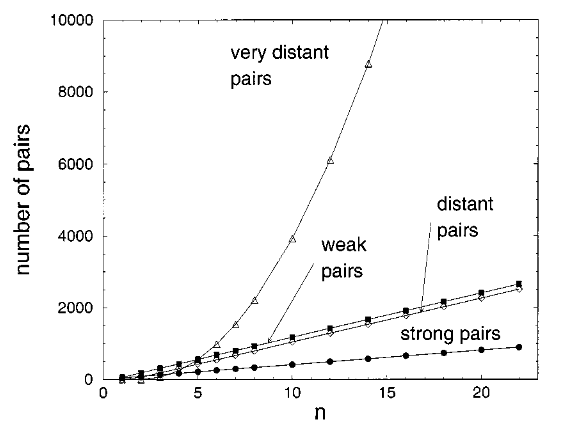
\includegraphics[scale=0.5]{Pics/electron_pairs.png}
\caption{Taken from Sch1999}
\end{figure}

\subsubsection{Linear Scaling LMP2}

It has been found [Sae1987] early on that the quadratic scaling very distant electron pairs can safely ignored without major impact on the total correlation energy. (Distance or Connectivity ciriteria) Distant pairs can also be approximated either by a multipole expansion (Het1998) or empirically (Rau1995), which further lowers the prefactor of the method. As a consequence, this establishes a sparsity relationship between $i$ and $j$, and the sparsity diagram for the MO integrals becomes fully connected
\begin{center}
\begin{tikzpicture}

\snode{MU}{0,0}{\mu};
\snode{SIG}{1,0}{\sigma};
\snode{NU}{2,0}{\nu};
\snode{LAM}{3,0}{\lambda};

\snode{I}{0,-1}{\uli};
\snode{A}{1,-1}{\ola};
\snode{J}{2,-1}{\ulj};
\snode{B}{3,-1}{\olb};

\draw[<->] (MU) -- (SIG) node [midway, above] () {S};
\draw[<->] (NU) -- (LAM) node [midway, above] () {S};
\draw[<->] (I) -- (MU) node [midway, below] () {};
\draw[<->] (A) -- (SIG) node [midway, below] () {};
\draw[<->] (J) -- (NU) node [midway, below] () {};
\draw[<->] (B) -- (LAM) node [midway, below] () {};
\draw[<->] (I) -- (A) node [midway, below] () {};
\draw[<->] (J) -- (B) node [midway, below] () {};
\draw[<->] (I) |- (1,-1.5) node [below] {$1/R^6$} -| (J);

\end{tikzpicture}
\end{center}
\noindent and linear scaling LMP2 therefore becomes possible (Sch1999).

% Sch1999 https://aip.scitation.org/doi/pdf/10.1063/1.479957

% distant pairs multipole approximate very distant pairs by multipole expansion Het1998 https://www.sciencedirect.com/science/article/pii/S0009261498004916

% distant pairs Empirically Rau1995 G. Rauhut, J. W. Boughton, and P. Pulay, J. Chem. Phys., 103, 5662 1995 .

Instead of using distance criteria, can use screening: 
%https://aip.scitation.org/doi/10.1063/1.4773581

\subsubsection{Density Fitting for LMP2}

While specific virtual orbitals form a very compact representation of the virtual space, the fact that each electron pair has their own orthogonal vitual orbital basis means that the total number of virtuals can become exceedingly large, and consequently increases the cost associated with the AO-MO transformation step. The most expensive step then becomes
\begin{equation}
\cn{\uli\ola}{P} = L_{\mu\uli} \cn{\mu\nu}{P} L_{\nu\ola}
\end{equation}
\noindent Transformation of the 3c2e integrals scales with $\ccpx{2}$. Linear scaling can be achieved by instroducing an orbital-specific fitting domain $[i]_fit$, e.g. by assigning all auxiliary functions $P$ on atoms with a Mulliken charge above a given threshold for the local orbital $i$ (Pin2015), or by using a Boughton-Pulay like scheme (Wer2015). This yields the sparsity diagramm
\begin{center}
\begin{tikzpicture}

\snode{P}{-1,0}{P};
\snode{MU}{0,0}{\mu};
\snode{SIG}{1,0}{\sigma};

\snode{I}{0,-1}{\uli};
\snode{A}{1,-1}{\ola};

\draw[<->] (MU) -- (SIG) node [midway, above] () {S};
\draw[<->] (I) -- (MU) node [midway, below] () {};
\draw[<->] (A) -- (SIG) node [midway, below] () {};
\draw[<->] (I) -- (A) node [midway, below] () {};
\draw[<->] (I) -- (-1,-1) node [below] {LDF} -- (P);

\end{tikzpicture}
\end{center}
\noindent As opposed to SOS-AO-MP2, where density fitting can give a more favourable factorization of the energy expression, the MO integrals need to fully assembled for LMP2 in order to solve the linear equations (...). The assembly is done in two steps
\begin{equation}
B^{X}_{\uli\ola} = \sum_{Y \in [i]_{fit} \cup [j]_{fit}} \cn{X}{Y}^{-1/2} \cn{Y}{\uli\ola}
\end{equation}
\begin{equation}
\cn{\uli\ola}{\ulj\olb} = \sum_{X \in [i]_{fit} \cup [j]_{fit}} B^{X}_{\uli\ola} B^{X}_{\ulj\olb} 
\end{equation}
\noindent The two steps are repeated for each electron pair $ij$, and the sum runs over all auxiliary functions $P$ in the unified fitting domain $[i]_{fit} \cup [j]_{fit}$, which enforces linear scaling for these steps as well. 

% Pin2015 https://aip.scitation.org/doi/pdf/10.1063/1.4926879
% Wer2015 https://pubs.acs.org/doi/pdf/10.1021/ct500725e

\subsection{Atomic Orbital Coupled Cluster}

\subsection{Local Coupled Cluster}

\subsection{FNO Coupled Cluster ??}

% Hylleraas functional: 
% Hyl1930 https://link.springer.com/article/10.1007/BF01397032

% First use of LMO+PNOs with Hylleraas 
% Pul1986 https://link.springer.com/article/10.1007%2FBF00526697

% LInear scaling of the functional
% Linear scaling of electron inetgrals
% linear scaling of MO-AO transformation -> or density fitting

